\textbf{\underline{OZ 7 - Inductantie - Oefening 4:}}
\vspace{0.5cm}

Op $t = 0$ wordt de open schakelaar gesloten. Toon aan door de regels van Kirchhoff te gebruiken dat de stroom in de spoel op $t > 0$ gelijk is aan:

\begin{equation*}
    I(t) = \frac{\mathcal{E}}{R_1} \left( 1 - e^{-\tfrac{R'}{L}t} \right)
\end{equation*}

waarbij $R' = \frac{R_1R_2}{R_1 + R_2}$.

\begin{center}
    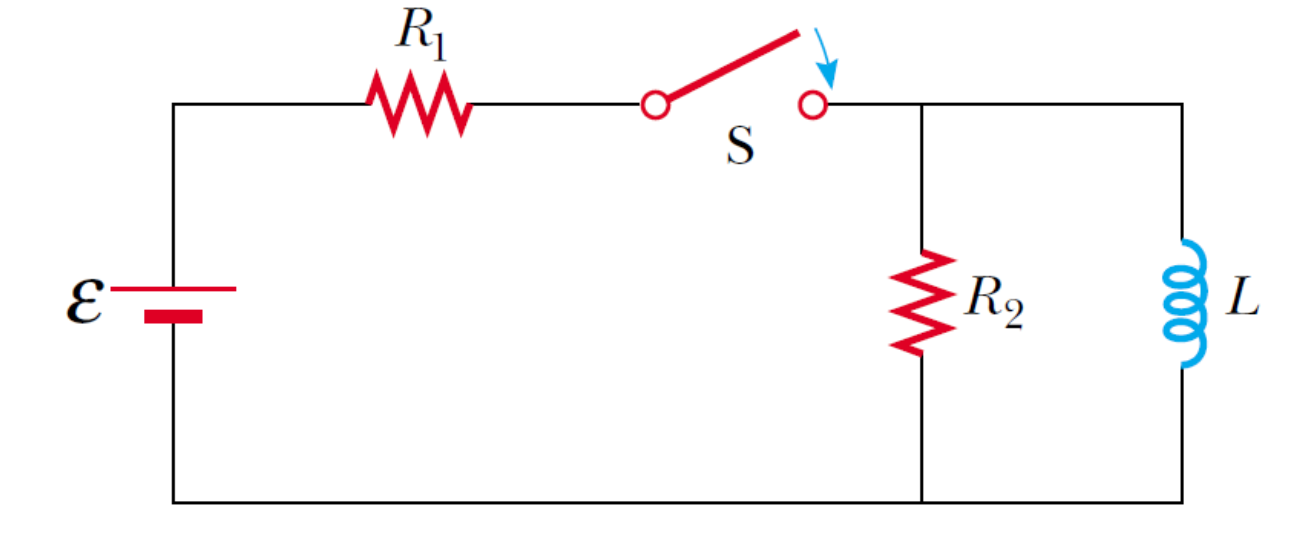
\includegraphics[scale = 0.3]{oz07/resources/Oz7Oef4.png}
\end{center}


\begin{description}[labelwidth=1.5cm, leftmargin=!]
    \item[Geg. :] 
    \item[Gevr. :] 
    \item[Opl. :]
\end{description}


\vspace{1cm}